\documentclass{article}
\usepackage{amsmath}
\usepackage{graphicx}

\begin{document}
$l_1c$ and $l_2c$ is the geometric center of links, and $l_1$ is the length of the link.
\begin{figure}
	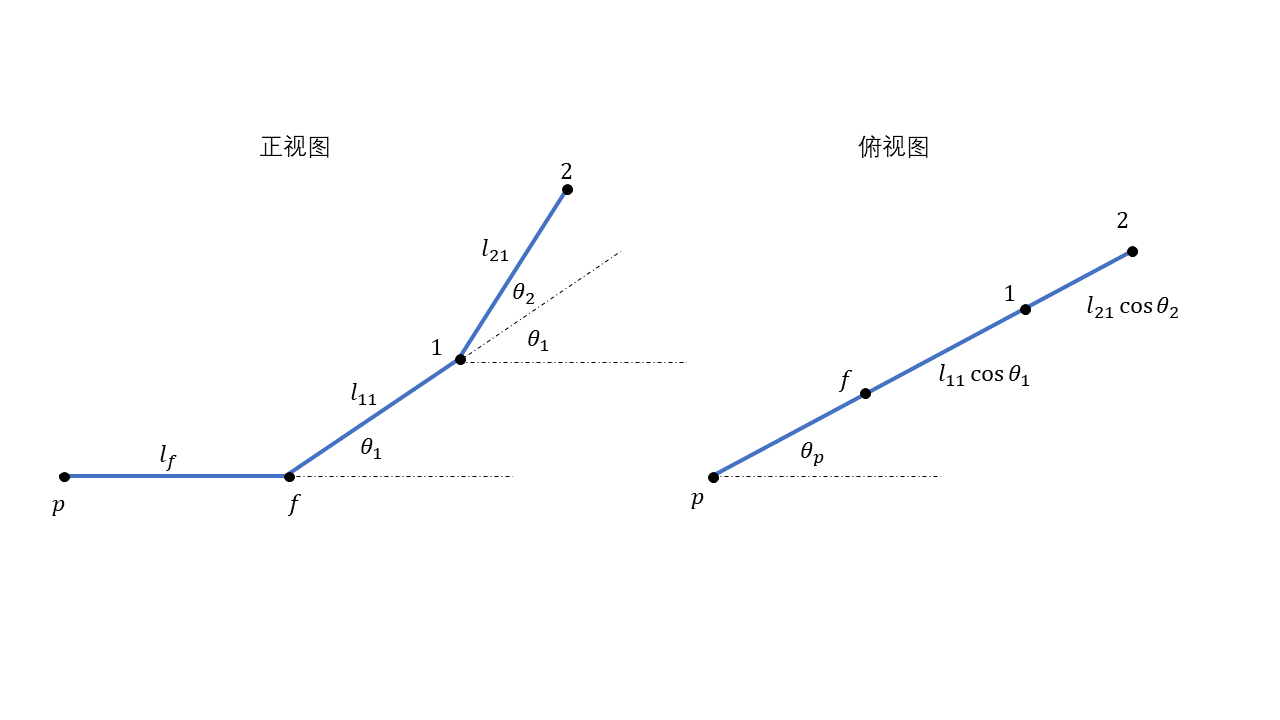
\includegraphics[width=\columnwidth]{./note}
	\centering
	\caption{
		note
	}
	\label{MoveError} 	
\end{figure} 

\begin{equation}
	\begin{aligned}
		x_f = x_p+l_f \cos \theta_p \\
		y_f = y_p+l_f \sin \theta_p \\
		z_f = 0		
	\end{aligned}
\end{equation}

\begin{equation}
	\begin{aligned}
		x_1 = x_f + l_{1c} \cos \theta_1 \cos \theta_p \\
		y_1 = y_f + l_{1c} \cos \theta_1 \sin \theta_p \\
		z_1 = l_{1c} \sin \theta_1
	\end{aligned}
\end{equation}

\begin{equation}
	\begin{aligned}
		x_1 = x_p+l_f \cos \theta_p + l_{1c} \cos \theta_1 \cos \theta_p \\
		y_1 = y_p+l_f \sin \theta_p + l_{1c} \cos \theta_1 \sin \theta_p \\
		z_1 = l_{1c} \sin \theta_1
	\end{aligned}
\end{equation}

\begin{equation}
	\begin{aligned}
		x_2 = x_p+l_f \cos \theta_p + (l_{1} \cos \theta_1 + l_{2c} \cos (\theta_1 + \theta_2) )\cos \theta_p \\
		y_2 = y_p+l_f \sin \theta_p + (l_{1} \cos \theta_1 + l_{2c} \cos (\theta_1 + \theta_2) )\sin \theta_p \\
		z_2 = l_{1} \sin \theta_1 + l_{2c} \sin (\theta_1 + \theta_2)
	\end{aligned}
\end{equation}

\begin{equation}
	\begin{aligned}
		\dot x_1 = \dot x_p - l_f \dot \theta_p \sin \theta_p - l_{1c} \dot \theta_1 \sin \theta_1 \cos \theta_p - l_{1c} \dot \theta_p \cos \theta_1 \sin \theta_p \\
		\dot y_1 = \dot y_p + l_f \dot \theta_p \cos \theta_p - l_{1c} \dot \theta_1 \sin \theta_1 \sin \theta_p + l_{1c} \dot \theta_p \cos \theta_1 \cos \theta_p \\
		z_1 = l_{1c} \dot \theta_1 \cos \theta_1
	\end{aligned}
\end{equation}

\begin{equation}
	\begin{aligned}
		\dot x_2 = \dot x_p - l_f \dot \theta_p \sin \theta_p - (l_{1} \dot \theta_1 \sin \theta_1+l_{2c} (\dot \theta_1 + \dot \theta_2) \sin (\theta_1 + \theta_2)) \cos \theta_p \\
		- \dot \theta_p(l_{1}  \cos \theta_1  + l_{2c}  \cos (\theta_1 + \theta_2)) \sin \theta_p \\
	   \dot y_2 = \dot y_p + l_f \dot \theta_p \cos \theta_p - (l_{1} \dot \theta_1 \sin \theta_1 + l_{2c} (\dot \theta_1 + \dot \theta_2) \sin (\theta_1 + \theta_2)) \sin \theta_p \\
		+ \dot \theta_p(l_{1}  \cos \theta_1  + l_{2c} \cos (\theta_1 + \theta_2)) \cos \theta_p \\
	   \dot z_2 = l_{1} \dot \theta_1 \cos \theta_1 + l_{2c} (\dot \theta_1 + \dot \theta_2) \cos (\theta_1 + \theta_2)
	\end{aligned}
\end{equation}

\begin{equation}
	\begin{aligned}
		E_0 = \frac{1}{2} m_0 (\dot x_p^2 + \dot y_p^2) + \frac{1}{2} I_0 \dot \theta_p^2	
	\end{aligned}
\end{equation}

\begin{equation}
	\begin{aligned}
		E_1 &= \frac{1}{2} m_1 (\dot x_1^2 + \dot y_1^2 + \dot z_1^2)=\frac{1}{2}m_1(\dot x_1^2 + \dot y_1^2 + l_{1c}^2 \dot \theta_1^2 \cos^2 \theta_1 ) \\
		&= \frac{1}{2} m_1 (l_{1c}^2 \dot \theta_p^2 \cos(\theta_1)^2 + 2 l_{1c} \dot \theta_p (\dot \theta_p l_f + \dot y_p \cos(\theta_p) - \dot x_p \sin(\theta_p)) \cos(\theta_1) \\
		&\quad  + (-2 l_{1c} \dot x_p \dot \theta_1 \sin(\theta_1) + 2 \dot y_p \dot \theta_p l_f) \cos(\theta_p) \\
		&\quad  + (-2 l_{1c} \dot y_p \dot \theta_1 \sin(\theta_1) - 2 \dot \theta_p l_f \dot x_p) \sin(\theta_p) + \dot \theta_p^2 l_f^2 + l_{1c}^2 \dot \theta_1^2 + \dot x_p^2 + \dot y_p^2)
	\end{aligned}
\end{equation}

\begin{equation}
	\begin{aligned}
		E_2 &= \frac{1}{2} m_2 (\dot \theta_p^2 (2 \cos(\theta_2)^2 l_{2c}^2 + 2 l_1 \cos(\theta_2) l_{2c} + l_1^2 - l_{2c}^2) \cos(\theta_1)^2 +\\
		&\quad  (-2 \dot \theta_p l_{2c} (\dot \theta_p \sin(\theta_2) l_{2c} \sin(\theta_1) - \dot \theta_p l_f - \dot y_p \cos(\theta_p) + \dot x_p \sin(\theta_p)) \cos(\theta_2) \\
		&\quad - 2 l_1 \dot \theta_p^2 \sin(\theta_1) \sin(\theta_2) l_{2c} + (-2 l_{2c} \dot x_p (\dot \theta_1 + \dot \theta_2) \sin(\theta_2) + 2 \dot y_p l_1 \dot \theta_p) \cos(\theta_p) \\
		&\quad - 2 \sin(\theta_p) l_{2c} \dot y_p (\dot \theta_1 + \dot \theta_2) \sin(\theta_2) + 2 l_1 \dot \theta_p (-\dot x_p \sin(\theta_p) + \dot \theta_p l_f)) \cos(\theta_1) - \\
		&\quad \cos(\theta_2)^2 l_{2c}^2 \dot \theta_p^2 + 2 (\dot \theta_1 + \dot \theta_2) ((-\cos(\theta_p) \dot x_p - \sin(\theta_p) \dot y_p) \sin(\theta_1) + l_1 \dot \theta_1) l_{2c} \cos(\theta_2)\\
		&\quad  + ((-2 \dot \theta_p \sin(\theta_2) l_{2c} \dot y_p - 2 \dot x_p l_1 \dot \theta_1) \cos(\theta_p) - 2 \dot \theta_p l_{2c} (-\dot x_p \sin(\theta_p) + \dot \theta_p l_f) \sin(\theta_2) \\
		&\quad - 2 l_1 \dot \theta_1 \sin(\theta_p) \dot y_p) \sin(\theta_1) + 2 \cos(\theta_p) \dot y_p l_f \dot \theta_p - 2 \sin(\theta_p) \dot x_p l_f \dot \theta_p \\
		&\quad + (\dot \theta_p^2 + (\dot \theta_1 + \dot \theta_2)^2) l_{2c}^2 + \dot \theta_1^2 l_1^2 + \dot \theta_p^2 l_f^2 + \dot x_p^2 + \dot y_p^2) 
	\end{aligned}
\end{equation}

\begin{equation}
	\begin{aligned}
	P = (l_1 m_2 + l_{1c} m_1) g \sin(\theta_1) + m_2 g l_{2c} \sin(\theta_1 + \theta_2)
	\end{aligned}
\end{equation}

$q=[x_p,y_p,\theta_p,\theta_1,\theta_2]^{\text{T}}$

\begin{equation}
	\begin{aligned}
		M(q)\ddot q + C(q,\dot q) \dot q + G(q) = N \tau
	\end{aligned}
\end{equation}
where,
\begin{equation}
	\begin{aligned}
		M = 
		\begin{bmatrix}
			M_v& M_{va} \\
			M_{av} & M_a
		\end{bmatrix}, C =
		\begin{bmatrix}
			C_v& C_{va} \\
			C_{av} & C_a
		\end{bmatrix}, G =
		\begin{bmatrix}
			G_v \\
			G_a
		\end{bmatrix}, N =
		\begin{bmatrix}
			N_v \\
			I_{2\times2}
		\end{bmatrix}
	\end{aligned}
\end{equation}

\begin{equation}
	\begin{aligned}
	G_v =
	\begin{bmatrix}
		0\\
		0 \\
		0 
	\end{bmatrix},N_v = \frac{1}{r}
	\begin{bmatrix}
		\cos(\theta_p)& 0 \\
		\sin(\theta_p)& 0 \\
		0 & \frac{b}{2}
	\end{bmatrix} 
	\end{aligned}
\end{equation}

\begin{equation}
	\begin{aligned}
	G_a =
	\begin{bmatrix}
		(l_1 m_2 + l_{1c} m_1) g \cos(\theta_1) + m_2 g l_{2c} \cos(\theta_1 + \theta_2)\\
		m_2 g l_{2c} \cos(\theta_1 + \theta_2)\\
	\end{bmatrix}
	\end{aligned}
\end{equation}


\begin{equation}
	\begin{aligned}
	M_v = 
	\begin{bmatrix}
		m_{11}& m_{12}& m_{13} \\
		m_{21}& m_{22}& m_{23} \\
		m_{31}& m_{32}& m_{33} \\
	\end{bmatrix},		M_{va} = 
	\begin{bmatrix}
		m_{14}& m_{15} \\
		m_{24}& m_{25} \\
		m_{34}& m_{35} \\
	\end{bmatrix}, \\
	M_{av} = 
	\begin{bmatrix}
		m_{41}& m_{42}& m_{43} \\
		m_{51}& m_{52}& m_{53} \\
	\end{bmatrix}, 	M_{a} = 
	\begin{bmatrix}
		m_{44}& m_{45} \\
		m_{54}& m_{55} \\
	\end{bmatrix}
	\end{aligned}
\end{equation}

\begin{equation}
	\begin{aligned}
		C_v = 
		\begin{bmatrix}
			c_{11} &c_{12} &c_{13} \\
			c_{21} &c_{22} &c_{23}   \\
			c_{31} &c_{32} &c_{33}   \\
		\end{bmatrix},			C_{va} = 
		\begin{bmatrix}
			c_{14}& c_{15} \\
			c_{24}& c_{25} \\
			c_{34}& c_{35} \\
		\end{bmatrix}, \\
		C_{av} = 
		\begin{bmatrix}
			c_{41}& c_{42}& c_{43} \\
			c_{51}& c_{52}& c_{53} \\
		\end{bmatrix}, 		C_{a} = 
		\begin{bmatrix}
			c_{44}& c_{45} \\
			c_{54}& c_{55} \\
		\end{bmatrix}
	\end{aligned}
\end{equation}

% 1
\begin{equation}
	\begin{aligned}
		m_{11} & = m_0 + m_1 + m_2 \\
		m_{12} & = 0\\
		m_{13} & = -(\cos(\theta_1 + \theta_2) l_{2c} m_2 + (l_1 m_2 + l_{1c} m_1) \cos(\theta_1) + l_f (m_1 + m_2)) sin(\theta_p) \\
		m_{14} & = -\cos(\theta_p) (sin(\theta_1) l_1 m_2 + sin(\theta_1) l_{1c} m_1 + \sin(\theta_1 + \theta_2) l_{2c} m_2)\\
		m_{15} & = -\cos(\theta_p) sin(\theta_1 + \theta_2) l_{2c} m_2\\
		c_{11} & = 0\\
		c_{12} & = 0\\
		c_{13} & = -\dot \theta_p \cos(\theta_p)(\cos(\theta_1 + \theta_2) l_{2c} m_2 + (l_1 m_2 + l_{1c} m_1) \cos(\theta_1) + l_f (m_1 + m_2))  \\
		&\quad + 2 \sin(\theta_p) (m_2 l_{2c} (\dot \theta_1 + \dot \theta_2) \sin(\theta_1 + \theta_2) + \dot \theta_1 \sin(\theta_1) (l_1 m_2 + l_{1c} m_1) )\\
		c_{14} & = - \dot \theta_1 \cos(\theta_p) ((\cos(\theta_2) m_2 l_{2c} + l_1 m_2 + l_{1c} m_1) \cos(\theta_1) - \sin(\theta_1) \sin(\theta_2) m_2 l_{2c})\\
		&\quad + \dot \theta_2 \cos(\theta_p) m_2 l_{2c} (\cos(\theta_1) \cos(\theta_2) - \sin(\theta_1)  \sin(\theta_2))  \\
		c_{15} & = \dot \theta_2 \cos(\theta_p) \cos(\theta_p) m_2 l_{2c} (\cos(\theta_1) \cos(\theta_2) - \sin(\theta_1) \sin(\theta_2))\\
		&\quad  + \dot \theta_1 \cos(\theta_p) m_2 l_{2c} (\cos(\theta_1) \cos(\theta_2) - \sin(\theta_1) \sin(\theta_2)) \\
	\end{aligned}
\end{equation}

% 2
\begin{equation}
	\begin{aligned}
		m_{21} & = 0 \\
		m_{22} & = m_0 + m_1 + m_2 \\
		m_{23} & = \cos(\theta_1 + \theta_2) \cos(\theta_p) l_{2c} m_2 + \cos(\theta_p) ((l_1 m_2 + l_{1c} m_1) \cos(\theta_1) + l_f (m_1 + m_2)) \\
		m_{24} & = -\sin(\theta_p) (\sin(\theta_1) l_1 m_2 + \sin(\theta_1) l_{1c} m_1 + \sin(\theta_1 + \theta_2) l_{2c} m_2) \\
		m_{25} & = -\sin(\theta_p) \sin(\theta_1 + \theta_2) l_{2c} m_2 \\
		c_{21} & = 0 \\
		c_{22} & = 0 \\
		c_{23} & = - \dot \theta_p \sin(\theta_p) ((l_1 m_2 + l_{1c} m_1) \cos(\theta_1) + l_f (m_1 + m_2)) \\
		&\quad -l_{2c} m_2 (\dot \theta_1 + \dot \theta_2) (\cos(\theta_p) + \cos(\theta_p)) \sin(\theta_1 + \theta_2) - 2 \cos(\theta_p) \sin(\theta_1) \dot \theta_1 (l_1 m_2 + l_{1c} m_1)\\
		c_{24} & = - \dot \theta_1 \sin(\theta_p) ((\cos(\theta_2) m_2 l_{2c} + l_1 m_2 + l_{1c} m_1) \cos(\theta_1) - \sin(\theta_1) \sin(\theta_2) m_2 l_{2c}) \\
		&\quad - \sin(\theta_p) \dot \theta_2 m_2 l_{2c} (\cos(\theta_1) \cos(\theta_2) - \sin(\theta_1) \sin(\theta_2))\\
		c_{25} & = - \dot \theta_2 \sin(\theta_p) m_2 l_{2c} (\cos(\theta_1) \cos(\theta_2) - \sin(\theta_1) \sin(\theta_2)) \\
		&\quad - \sin(\theta_p) m_2 l_{2c} (\cos(\theta_1) \cos(\theta_2) - \sin(\theta_1) \sin(\theta_2)) \dot \theta_1\\
	\end{aligned}
\end{equation}

% 3
\begin{equation}
	\begin{aligned}
		m_{31} & =  (\cos(\theta_1 + \theta_2) l_{2c} m_2 + (l_1 m_2 + l_{1c} m_1) \cos(\theta_1) + l_f (m_1 + m_2)) \cos(\theta_p) \\
		m_{32} & = -(\cos(\theta_1 + \theta_2) l_{2c} m_2 + (l_1 m_2 + l_{1c} m_1) \cos(\theta_1) + l_f (m_1 + m_2)) \sin(\theta_p) \\
		m_{33} & = \cos(\theta_1 + \theta_2)^2 l_{2c}^2 m_2 + 2 m_2 l_{2c} (l_1 \cos(\theta_1) + l_f) \cos(\theta_1 + \theta_2) \\
		& \quad + (l_1^2 m_2 + l_{1c}^2 m_1) \cos(\theta_1)^2 + 2 l_f (l_1 m_2 + l_{1c} m_1) \cos(\theta_1) + l_f^2 m_1 + l_f^2 m_2 + I_0 \\
		m_{34} & = 0 \\
		m_{35} & = 0 \\
		c_{31} & = \sin(\theta_p) (\sin(\theta_2) m_2 l_{2c} (\dot\theta_1 + \dot\theta_2) \cos(\theta_1) \\
		& \quad + \sin(\theta_1) (m_2 l_{2c} (\dot\theta_1 + \dot\theta_2) \cos(\theta_2) + \dot\theta_1 (l_1 m_2 + l_{1c} m_1))) \\
		& \quad -\cos(\theta_p) ((\cos(\theta_2) m_2 l_{2c} + l_1 m_2 + l_{1c} m_1) \cos(\theta_1) - \sin(\theta_1) \sin(\theta_2) m_2 l_{2c} \\
		& \quad + l_f (m_1 + m_2)) \dot \theta_p + ((\cos(\theta_1) \sin(\theta_2) m_2 l_{2c} + \sin(\theta_1) (\cos(\theta_2) m_2 l_{2c} + l_1 m_2 + l_{1c} m_1)) \dot \theta_1 \\
		& \quad + \dot \theta_2 m_2 l_{2c} (\sin(\theta_1) \cos(\theta_2) + \cos(\theta_1) \sin(\theta_2))) \sin(\theta_p) \\
		c_{32} & = -\cos(\theta_p)(\sin(\theta_2) m_2 l_{2c} (\dot\theta_1 + \dot\theta_2) \cos(\theta_1) \\
		& \quad + \sin(\theta_1) (m_2 l_{2c} (\dot\theta_1 + \dot\theta_2) \cos(\theta_2) + \dot\theta_1 (l_1 m_2 + l_{1c} m_1))) \\
		&\quad -((\cos(\theta_2) m_2 l_{2c} + l_1 m_2 + l_{1c} m_1) \cos(\theta_1) - \sin(\theta_1) \sin(\theta_2) m_2 l_{2c} \\
		& \quad + l_f (m_1 + m_2)) \sin(\theta_p) \dot \theta_p - ((\cos(\theta_1) \sin(\theta_2) m_2 l_{2c} + \sin(\theta_1) (\cos(\theta_2) m_2 l_{2c} + l_1 m_2 + l_{1c} m_1)) \dot \theta_1 \\
		& \quad + \dot \theta_2 m_2 l_{2c} (\sin(\theta_1) \cos(\theta_2) + \cos(\theta_1) \sin(\theta_2))) \cos(\theta_p) \\
		c_{33} & = -m_2 l_{2c}^2 (\dot \theta_1 + \dot \theta_2) \sin(2 \theta_1 + 2 \theta_2) - 2 l_1 l_{2c} (\dot \theta_1 + \dot \theta_2/2) m_2 \sin(\theta_2 + 2 \theta_1) \\
		& \quad - 2 l_f m_2 l_{2c} (\dot \theta_1 + \dot \theta_2) \sin(\theta_1 + \theta_2) - \dot \theta_1 (l_1^2 m_2 + l_{1c}^2 m_1) \sin(2 \theta_1) \\
		& \quad - 2 \sin(\theta_1) l_f (l_1 m_2 + l_{1c} m_1) \dot \theta_1 - \sin(\theta_2) \dot \theta_2 l_1 m_2 l_{2c} \\
		&\quad \\
		c_{34} & =  0 \\
		&\quad  \\
		c_{35} & =  0 \\
		&\quad  \\
	\end{aligned}
\end{equation}

% 4
\begin{equation}
	\begin{aligned}
		m_{41} & = -((cos(theta__2(t))*m__2*l__21 + l__1*m__2 + m__1*l__11)*sin(theta__1(t)) + cos(theta__1(t))*sin(theta__2(t))*m__2*l__21)*cos(theta__p(t)) \\
		m_{42} & = -((cos(theta__2(t))*m__2*l__21 + l__1*m__2 + m__1*l__11)*sin(theta__1(t)) + cos(theta__1(t))*sin(theta__2(t))*m__2*l__21)*sin(theta__p(t)) \\
		m_{43} & = 0 \\
		m_{44} & = 2*cos(theta__2(t))*l__1*m__2*l__21 + (l__1^2 + l__21^2)*m__2 + m__1*l__11^2 \\
		m_{45} & = m__2*l__21*(cos(theta__2(t))*l__1 + l__21) \\
		c_{41} & = 0 \\
		c_{42} & = 0 \\
		c_{43} & = ((cos(theta__2(t))*m__2*l__21 + l__1*m__2 + m__1*l__11)*sin(theta__1(t)) + cos(theta__1(t))*sin(theta__2(t))*m__2*l__21)*(diff(x__p(t), t)*sin(theta__p(t)) - diff(y__p(t), t)*cos(theta__p(t))) \\
		c_{44} & =  -2*sin(theta__2(t))*l__1*m__2*l__21*diff(theta__2(t), t) - (-sin(theta__2(t))*m__2*l__21*sin(theta__1(t)) + cos(theta__1(t))*(cos(theta__2(t))*m__2*l__21 + l__1*m__2 + m__1*l__11))*(diff(x__p(t), t)*cos(theta__p(t)) + diff(y__p(t), t)*sin(theta__p(t))) \\
		c_{45} & =  -m__2*l__21*(sin(theta__2(t))*l__1*diff(theta__2(t), t) + (cos(theta__1(t))*cos(theta__2(t)) - sin(theta__1(t))*sin(theta__2(t)))*(diff(x__p(t), t)*cos(theta__p(t)) + diff(y__p(t), t)*sin(theta__p(t)))) \\
	\end{aligned}
\end{equation}

% 5
\begin{equation}
	\begin{aligned}
		m_{51} & =   \\
		m_{52} & =  \\
		m_{53} & =  \\
		m_{55} & =  \\
		c_{51} & =  \\
		c_{52} & =  \\
		c_{53} & =  \\
		&\quad \\
		c_{54} & =   \\
		&\quad  \\
		c_{55} & =   \\
		&\quad  \\
	\end{aligned}
\end{equation}
\end{document}